\documentclass[conference]{IEEEtran}
\IEEEoverridecommandlockouts
% The preceding line is only needed to identify funding in the first footnote. If that is unneeded, please comment it out.
\usepackage{cite}
\usepackage{amsmath,amssymb,amsfonts}
\usepackage{algorithmic}
\usepackage{graphicx}
\usepackage{textcomp}
\usepackage{xcolor}
\usepackage{subfig}
\def\BibTeX{{\rm B\kern-.05em{\sc i\kern-.025em b}\kern-.08em
    T\kern-.1667em\lower.7ex\hbox{E}\kern-.125emX}}
\begin{document}

\title{HDR Tone Mapping\\{\LARGE Trabalho Final PDI}}

\author{\IEEEauthorblockN{Frederico Peixoto Antunes}
\IEEEauthorblockA{\textit{CDTec - Ciência da Computação} \\
\textit{UFPel}\\
Pelotas, Brazil \\
fpantunes@inf.ufpel.edu.br}
\and
\IEEEauthorblockN{José Felipe Moré Pauletti}
\IEEEauthorblockA{\textit{CDTec - Ciência da Computação} \\
\textit{UFPel}\\
Pelotas, Brazil \\
jfmpauletti@inf.ufpel.edu.br}
}

\maketitle

\begin{abstract}
The vast majority of camera sensors and digital displays don't have the capability to capture or display the full range of colors the human eye can perceive. The technical limitations that only allow these cameras to capture a small range of the full electromagnetic waves result on images of Low Dynamic Range (LDR), which are limited to 255 levels of luminance for each color channel and are the images we are used to seeing on most situations.

With the technological development, the hardware and software capabilities to capture and process a broader range of colors on a single image became more accessible, and with that came the development of High Dynamic Range (HDR), which are digital images capable to storing more information about the luminance and color of a picture.

Even with the bigger access to HDR compatible hardware, most displays are still limited to the LDR color range, and, as there are different ranges to HDR, even the ones compatible might not be able to output the full scope of a given image. To solve that problem tone-mapping techniques are used to map the full range of HDR colors to the limited capacity of LDR pictures, these techniques are commonly called Tone Mapping Operators.

This paper was done as a final activity for the Digital Image Processing course, with the objective of using the knowledge acquired during the semester to implement and analyze at least two different different Tone Mapping Operators (TMO). In the end four different operators were implemented (Logarithmic, Modified Logarithmic, Eponential and Modified Exponential), and a Tone Mapping Quality Index (TMQI) function was used to acquire an objective assessment on the results.
\end{abstract}

\begin{IEEEkeywords}
HDR, Tone Mapping, Image Processing
\end{IEEEkeywords}

\section{Introdução}

O uso de câmeras fotográficas digitais, nos permite realizar edições e a solucionar possíveis problemas gerados na hora da fotografia. Atualmente um dos métodos mais conhecidos para tratar de problemas de iluminação é o \textit{High Dynamic Range} (HDR), que permite ampliar a faixa dinâmica de cores de uma determinada imagem. Com esse aumento da popularidade, tanto pelos setores da industria fotográfica quanto pelos setores de pesquisa acadêmica, houve um aumento nos estudos e desenvolvimento de algoritmos para ampliar a faixa dinâmica.

No entanto, os dispositivos que temos disponíveis, não são capazes de representar a luminosidade de uma cena real, por isso foi desenvolvido o método de \textit{Tone Mapping}, no qual torna capaz a visualização da maior quantidade de detalhes de uma imagem HDR nos limites estabelecidos por imagens \textit{Low Dynamic Range} (LDR). \cite{ICIAS}

Na Figura \ref{TM}, é possível visualizar uma imagem com o tratamento por meio do \textit{Tone Mapping}, onde a imagem HDR perde muitos detalhes e ficando muito difícil de se ver detalhes.

\begin{figure}[!htpb]
    \centering
    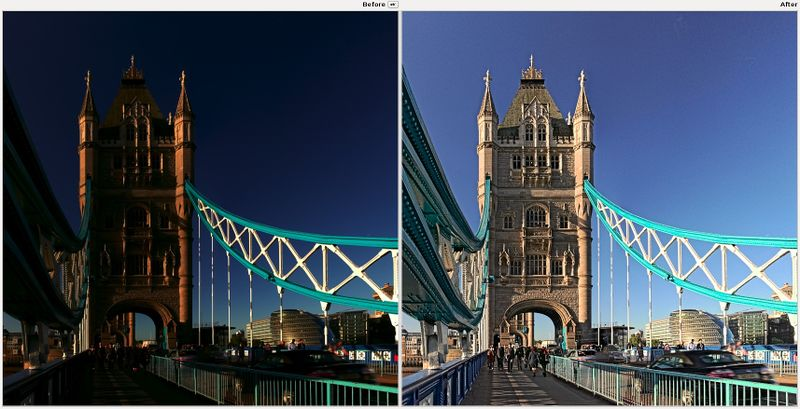
\includegraphics[scale=.20]{Imagens/hdrldr.jpg}
    \caption{Imagem com o uso de Tone Mapping para melhor visualização \cite{RawPedia}}
    \label{TM}
\end{figure}

Ao gerar uma imagem HDR, acabamos tendo uma dificuldade de visualizar essa imagem, por causa do grande intervalo de luminosidade. Para isso, podemos utilizar o método de \textit{Tone Mapping}, no qual nos permite visualizar essas variações.
A implementação destes processos pode ser feita utilizando um de dois métodos, métodos globais ou métodos locais, onde no método global o processo não ajusta a luminosidade por áreas, mas sim faz um ajuste da luminosidade dos \textit{pixeis} da imagem toda de forma uniforme. O método local propõem a ideia de tratar a segmentação de regiões da imagem e ajustar as cores usando os máximos e mínimos locais.

Neste trabalho são apresentados quatro implementações diferentes de \textit{Tone Mapping}, sendo todas elas parte do conjunto de algoritmos de Tone Mapping que utilizam do método global, e são elas os operadores Logarítmico, Exponencial e a versão modificada de ambas, podendo assim realizar uma comparação, em qual delas temos uma imagem resultante com melhores cores, maior clareza dos detalhes em todas as áreas da imagem e, de forma geral, uma imagem mais visualmente agradável. %$Para isso foram enviadas duas imagens para 10 pessoas, sendo a imagem HDR original e o resultado de cada algoritmo.   
%Acho que a explicação da metodologia de avaliação pode ir só nos resultados, e de qualquer maneira essa frase em específica ficou estranha

\section{Metodologia Empregada}

Para realizar a implementação Operadores de Tone Mapping (TMO), que utilizam diferentes métodos para obter uma melhor visualização LDR de imagens HDR , foi utiliza o programa Octave. Além disso também foi necessário a instalação de uma biblioteca/ferramente de terceiros que permitisse a leitura e manipulação de imagens HDR, tendo em vista que as funções para tal somente existem nas bibliotecas do programa MatLab e ainda não foram implementadas para o Octave. A ferramenta escolhida e instalada para obter acesso à funções de HDR foi a HDR\_Toolbox \cite{Banterle:2017}.

Esta ferramente foi utilizada neste trabalho majoritariamente para ser possível fazer-se a leitura das imagens HDR, com o uso da função \textit{hdrimread} disponibilizada por ela. O código fonte que acompanha os arquivos da ferramenta também foram de grande utilidade para preencher lacunas na compreensão da implementação causados por equívocos e formas estranhas de implementação presentes em outros artigos e trabalhos.

A HDR\_Toolbox também foi utilizada em uma menor escala na implementação com o uso das funções prontas disponibilizadas, que permitiram mais facilmente encontrar trechos do código que estavam causando problema, e comparar o resultado final da implementação com o resultado retornado pelas funções, validando o que foi desenvolvido.

Com o acesso à ferramenta foi então possível finalmente testar, corrigir e implementar partes que faltavam dos Operadores de Tone Mapping, os quais já estavam parcialmente implementados mas não funcionais pelas limitações do Octave.

Os quatro operadores que acabaram sendo implementados para o trabalho foram o Logarítmico, o Logarítmico Modificado, o Exponencial e o Exponencial Modificado.

\subsection{Logarítmico (LTM)}

O operador logarítmico consiste de três principais etapas, como pode ser observado na Figura \ref{LTM}.

A primeira parte de todos operadores desenvolvidos envolve o cálculo da luminância da imagem obtida através da média ponderada da luminância de cada um dos canais de cores da imagem.

A segunda parte consiste do cálculo da nova luminância à ser usada para a imagem através do uso da função logarítmica no valor da luminância, obtida na etapa um, e no valor da luminância máxima, obtida com o maior valor entre cada pixel individual.

A terceira parte é onde é feito algoritmo de correção gamma onde são feitos cálculos entre as luminâncias de cada canal de cor e as luminâncias obtidas nas etapas anteriores para comprimir cada em um canal RGB da imagem e obter a imagem LDR final.

\begin{figure}[!htpb]
    \centering
    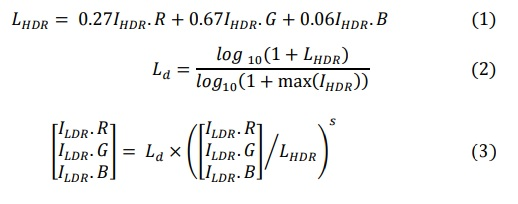
\includegraphics[scale=.40]{Imagens/log.jpg}
    \caption{Equações do Operador Logarítmico}
    \label{LTM}
\end{figure}

Na Figura \ref{LTM2} se apresenta o trecho de código que e se refere unicamente à implementação do operador logarítmico, sendo possível inclusive observar que o nome de algumas variáveis destoam dos nomes utilizados nas fórmulas, isso tendo sido feito para uma mais fácil leitura e compreensão da implementação.

\begin{figure}[!htpb]
    \centering
    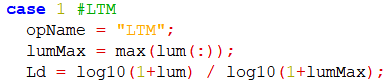
\includegraphics[scale=.40]{Imagens/ltmcod2.png}
    \caption{Código do Operador Logarítmico}
    \label{LTM2}
\end{figure}

\subsection{Logarítmico Modificado(MLTM)}

O operador logarítmico modificado é extremamente semelhante ao logarítmico já apresentado, exatamente como o nome indica.

O MLTM se distingue do LTM na forma que a luminância é calculada, sendo feito o cálculo individualmente para cada um dos canais RGB da imagem, tal qual pode ser visto na Figura \ref{MLTM}. Isso então acaba por também modificar ligeiramente o cálculo usado para comprimir todas luminâncias nos canais RGB da imagem final.

\begin{figure}[!htpb]
    \centering
    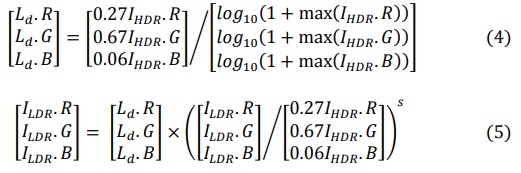
\includegraphics[scale=.40]{Imagens/logm.jpg}
    \caption{Equações do Operador Logarítmica Modificado}
    \label{MLTM}
\end{figure}

Essa aparente pequena modificação acaba sendo mais perceptível na implementação, como visto na Figura \ref{MLTM2}, sendo necessário o uso de laços, adição de variáveis, além de algumas outras modificações no código que não podem ser vistas na figura porém afetaram a estrutura do código como um todo, e não somente o segmento específico do MLTM.

\begin{figure}[!htpb]
    \centering
    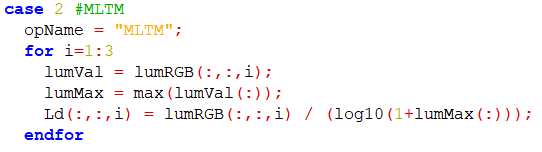
\includegraphics[scale=.40]{Imagens/mltmcod.png}
    \caption{Código do Método Logarítmica Modificado}
    \label{MLTM2}
\end{figure}

\subsection{Exponencial(ETM)}

A operação exponencial em muito se assemelha com a logarítmica, fora a óbvia distinção do uso da função exponencial no lugar da logarítmica. 

Ambas usam o mesmo cálculo de luminância RGB e cálculo de correção gamma como vistos na Figura \ref{LTM}.
Porém a nova luminância a ser usada para a imagem é calculada com o uso do ganho exponencial em cima de um valor médio da luminância que deve ser calculado, como demonstrado na Figura \ref{ETM}.

\begin{figure}[!htpb]
    \centering
    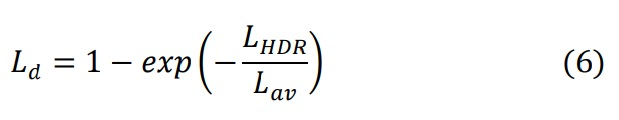
\includegraphics[scale=.45]{Imagens/etm.jpg}
    \caption{Equação do Operador Exponencial}
    \label{ETM}
\end{figure}

Na implementação do código dessa operação é onde vem o maior trabalho de entender como fazer essa operação funciona, com a necessidade de primeiro se obter um delta para aí então poder se conseguir a média da luminância necessária para o cálculo.

Esse cálculo do delta e da média podem ser vistos na Figura \ref{ETM2}. Além disso o resto do código se assemelha muito ao do LTM, e portanto pode ser reutilizado.

\begin{figure}[!htpb]
    \centering
    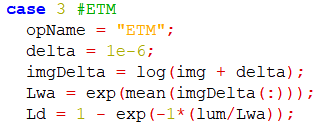
\includegraphics[scale=.45]{Imagens/etmcod.png}
    \caption{Código do Operador Exponencial}
    \label{ETM2}
\end{figure}

\subsection{Exponencial Modificado(METM)}

A operação exponencial modificada é a que menos possui o que se comentar, pois ela utiliza os mesmos princípios já explicados em operações anteriores, sendo o método exponencial da ETM com as mesmas modificações feitas na MLTM.

No código essa semelhança com as operações previamente explicadas e implementadas também é extremamente visível (Figura \ref{METM}), sendo apenas o mesmo código do exponencial dentro da estrutura de laço do logarítmico modificado. As modificações necessárias no resto do código para o MLTM também podem ser reutilizadas, não sendo necessário fazer mais nada no código.

\begin{figure}[!htpb]
    \centering
    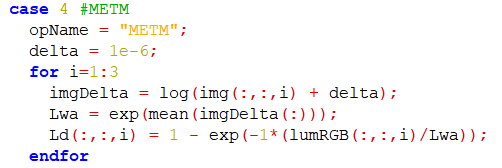
\includegraphics[scale=.45]{Imagens/metmcod.png}
    \caption{Código do Operador Exponencial Modificado}
    \label{METM}
\end{figure}


\section{Resultados e Discussão}

Após a implementação do algoritmo dos operadores, foram baixadas imagens nos formatos \textit{.hdr} e \textit{.exr} de dois datasets de imagens HDR \cite{Mantiuk:2007} \cite{HDR_Dataset}. As 10 imagens selecionadas dos datasets, juntamente com uma imagem adicional \textit{.hdr} que faz parte da ferramente HDR Toolbox, foram usadas na execução do \textit{Tone Mapping} implementado. Após o tratamento, cada imagem gerada foi colocada lado a lado, foram realizados testes visuais com o objetivo de visualizar os efeitos do tone mapping na imagem final, e avaliar de forma subjetiva qual atingia um resultado mais claro e agradável. Também foi feita uma avaliação com fatores objetivos, que utilizou a função Tone Mapping Quality Index (TMQI) \cite{TMQI} disponibilizada no pacote de ferramentas do HDR\_Toolbox. A análise do TMQI faz a avaliação com base de fatores como fidelidade estrutural da imagem LDR, grau de naturalidade estatística da imagem LDR e uma pontuação TMQI geral dada para a imagem.

É possível verificar que ao ser passados pelos algoritmos, obtivemos os melhores resultados no uso do operador LTM, tanto na análise subjetiva quanto nos valores obtidos pela análise objetiva. Durante os testes foi possível verificar que os algoritmos de METM apresentaram um erro no qual as imagens ficaram com uma tonalidade mais arroxeada, e que os método MLTM apresentaram um problema no qual o branco passa a predominar na imagem, perdendo, assim, os seus detalhes.

\begin{figure}[!htp]
   \centering
  \subfloat[ETM]{\label{fig:ETM}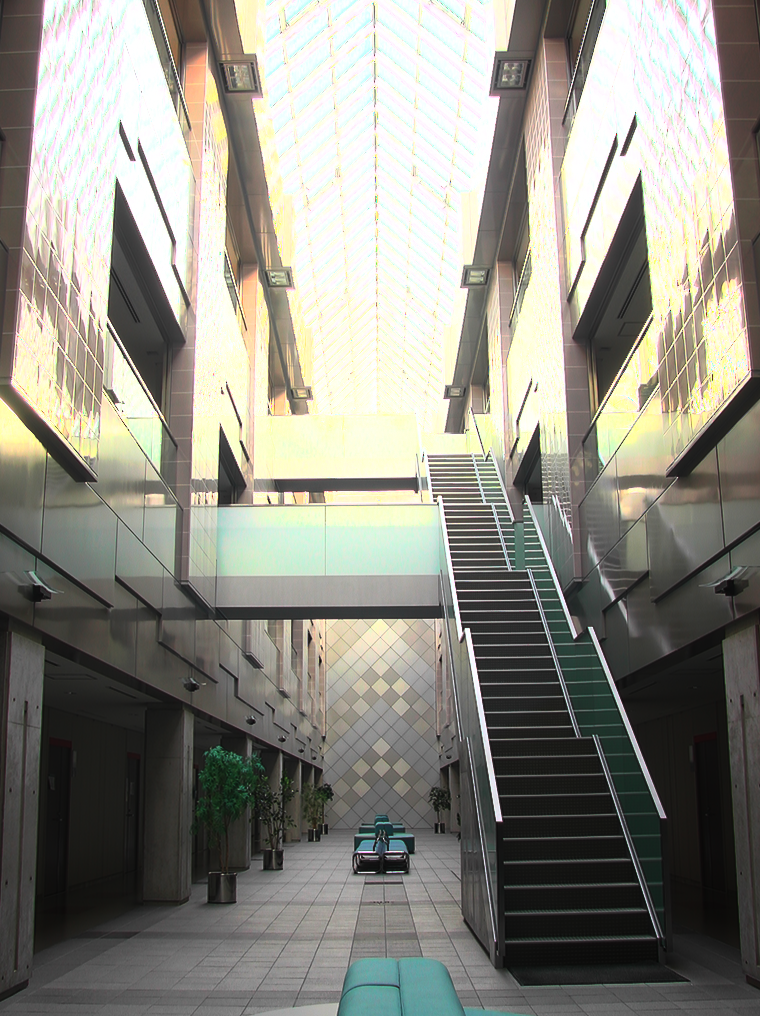
\includegraphics[height=1.5cm]{Imagens/AtriumMorning-ETM.png}}
    \hspace{0.3cm}
  \subfloat[METM]{\label{fig:METM} 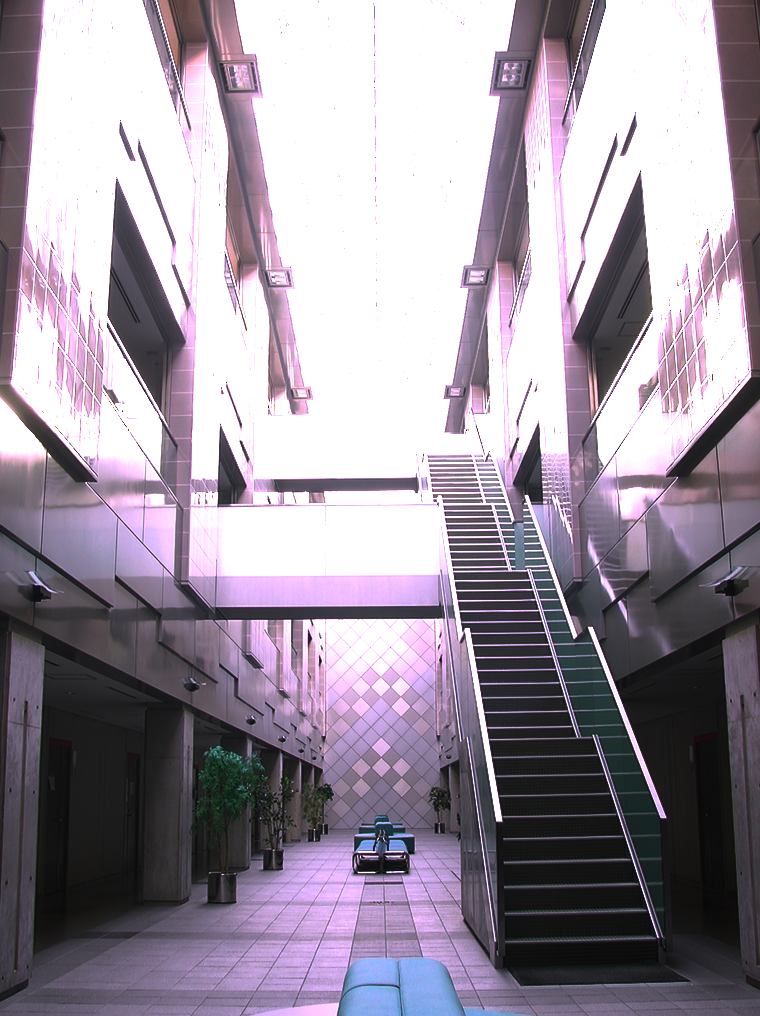
\includegraphics[height=1.5cm]{Imagens/AtriumMorning-METM.png}}
  \hspace{0.3cm}
   \subfloat[LTM]{\label{fig:LTM}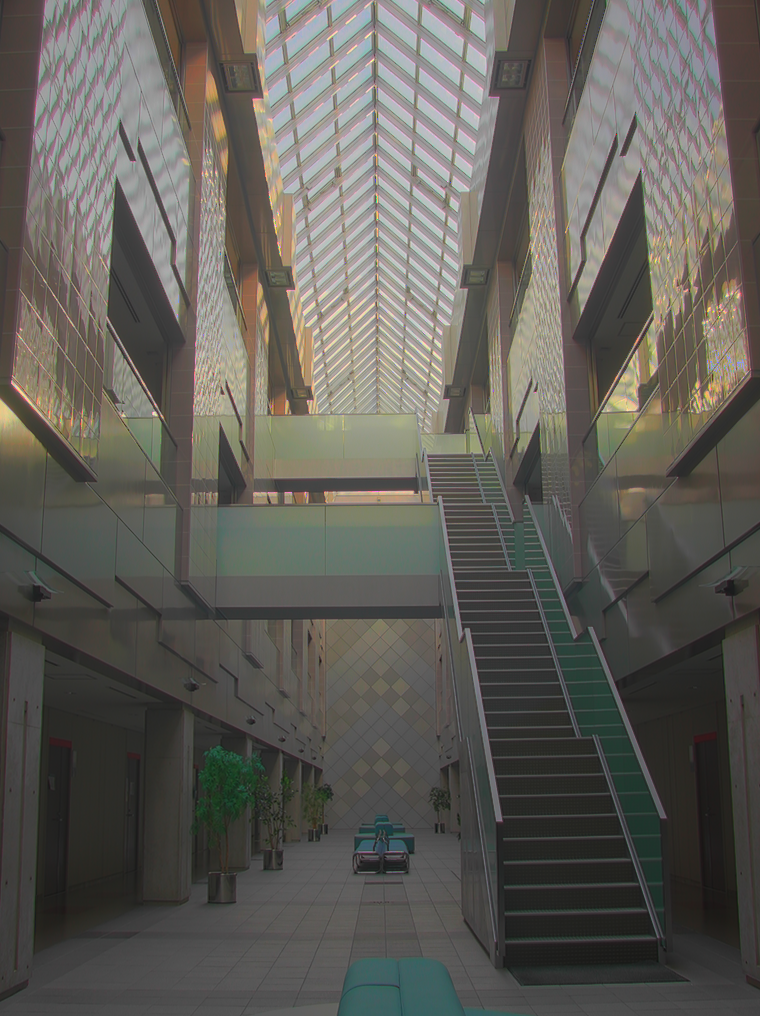
\includegraphics[height=1.5cm]{Imagens/AtriumMorning-LTM.png}}
    \hspace{0.3cm}
   \subfloat[MLTM]{\label{fig:MLTM}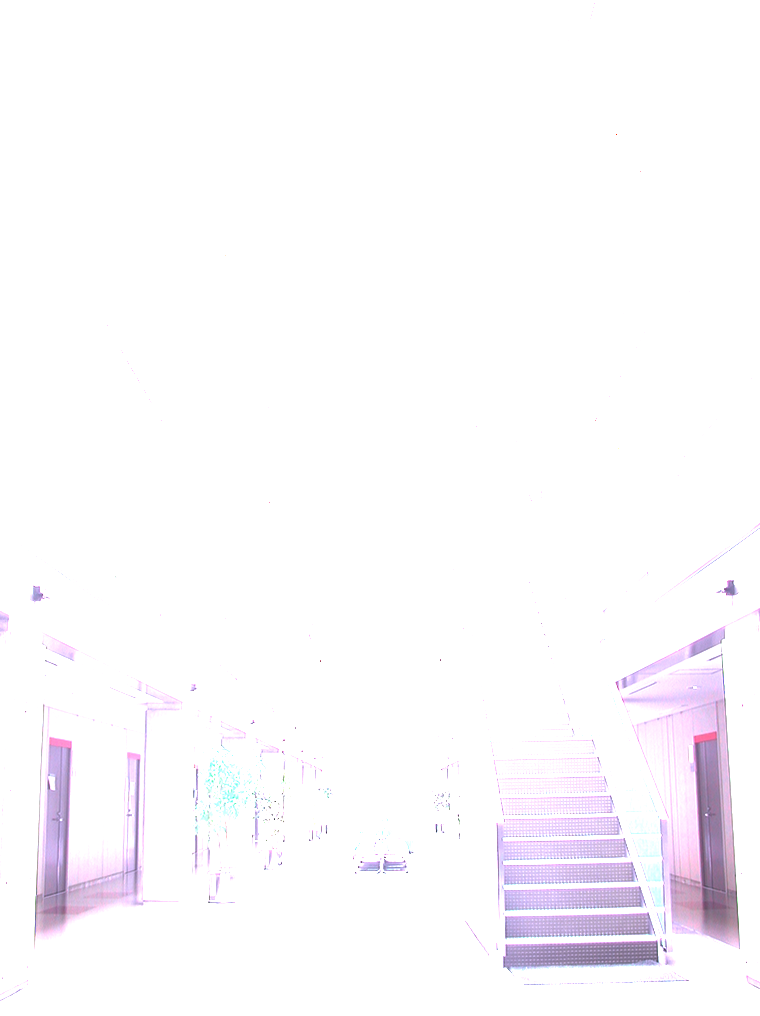
\includegraphics[height=1.5cm]{Imagens/AtriumMorning-MLTM.png}}
    \caption{Atrium Morning \cite{HDR_Dataset}}
    \label{fig:atMorn}
\end{figure}

\begin{figure}[!htp]
   \centering
  \subfloat[ETM]{\label{fig:ETM}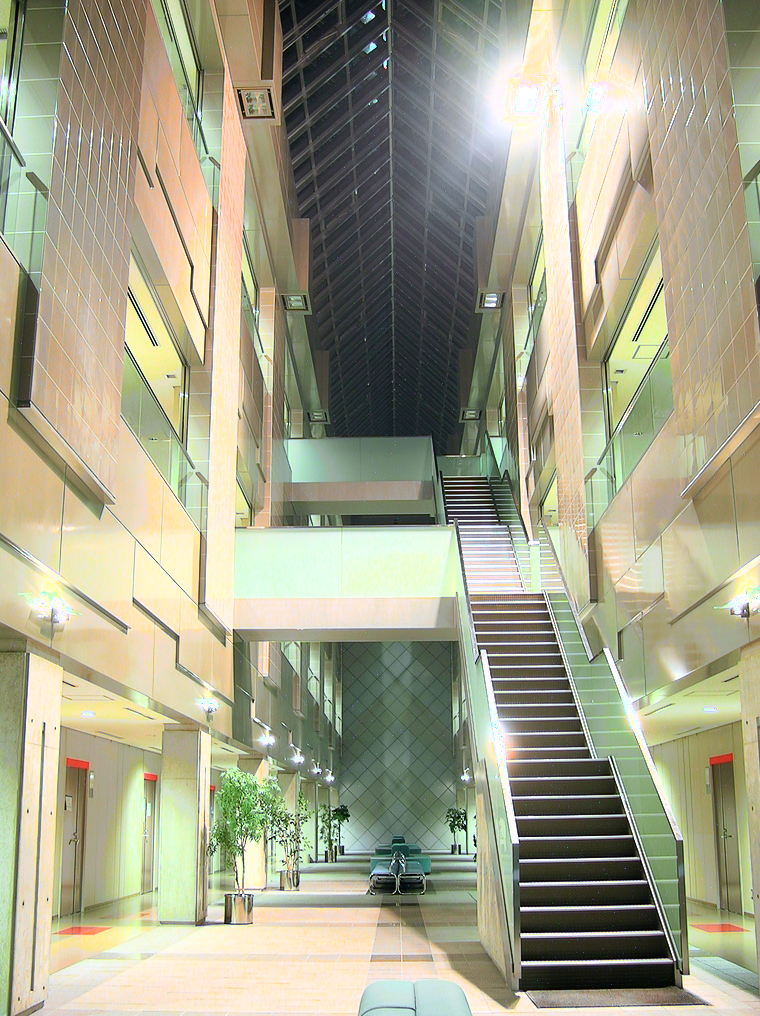
\includegraphics[height=1.5cm]{Imagens/AtriumNight-ETM.png}}
    \hspace{0.3cm}
  \subfloat[METM]{\label{fig:METM} 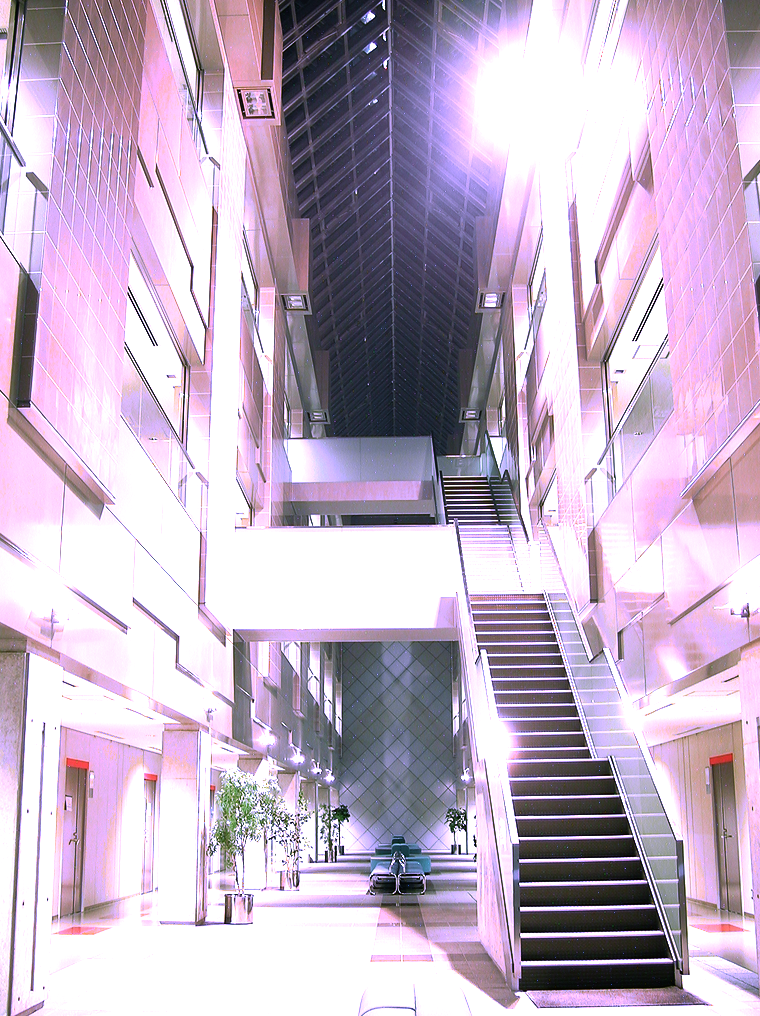
\includegraphics[height=1.5cm]{Imagens/AtriumNight-METM.png}}
  \hspace{0.3cm}
   \subfloat[LTM]{\label{fig:LTM}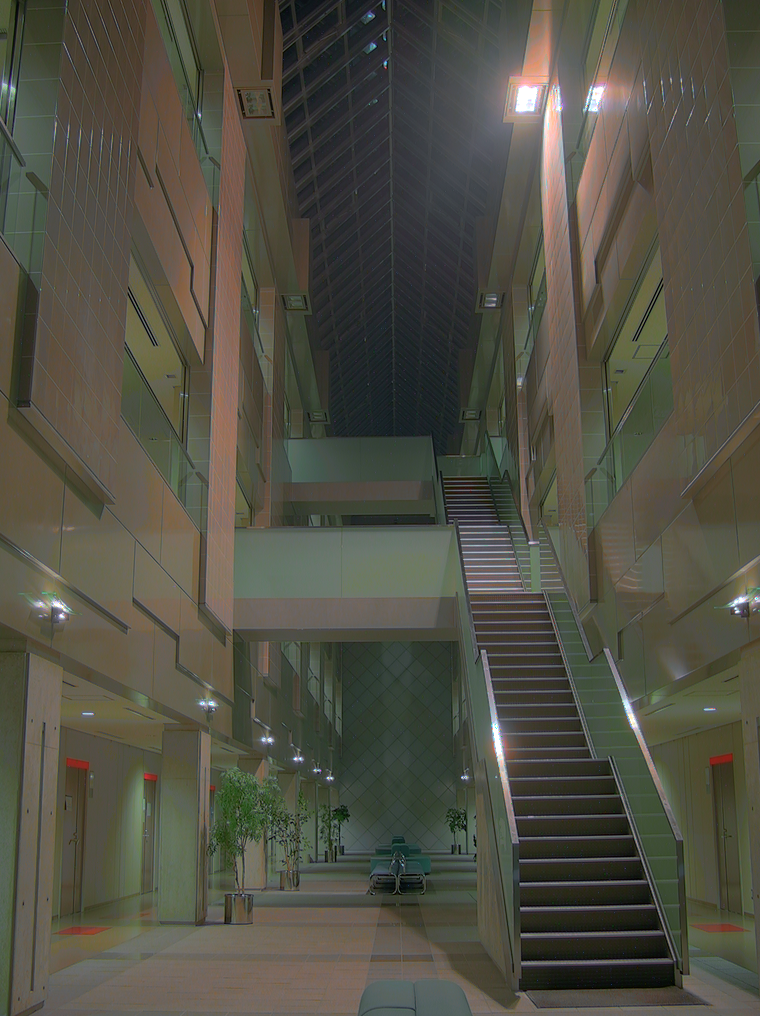
\includegraphics[height=1.5cm]{Imagens/AtriumNight-LTM.png}}
    \hspace{0.3cm}
   \subfloat[MLTM]{\label{fig:MLTM}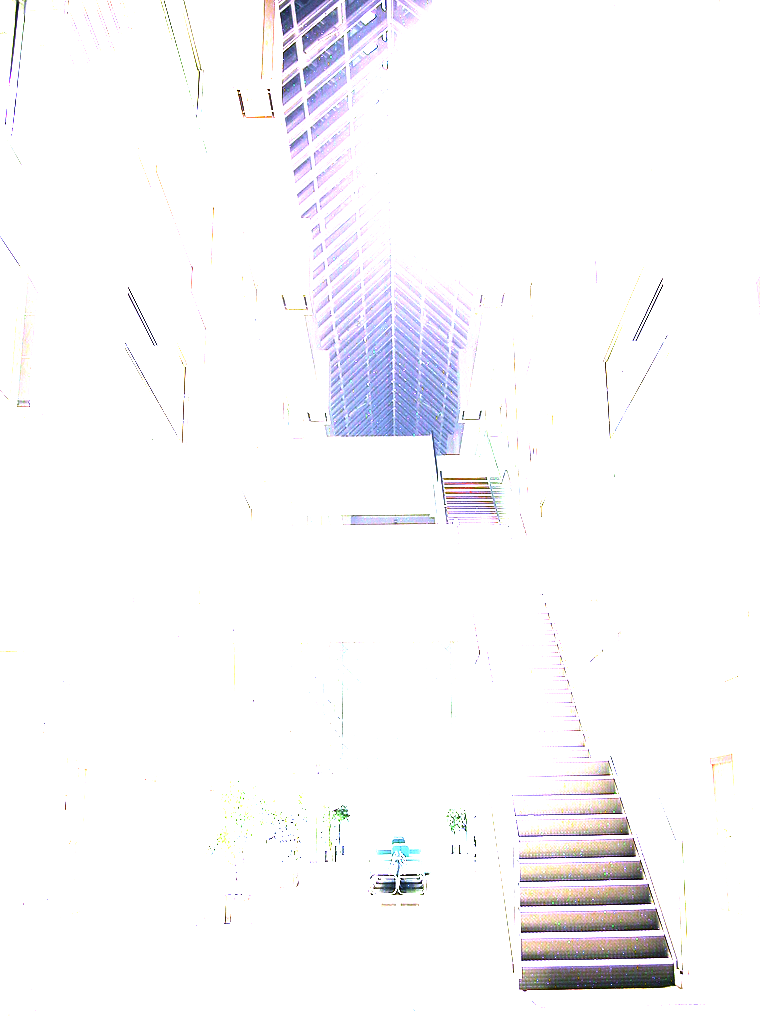
\includegraphics[height=1.5cm]{Imagens/AtriumNight-MLTM.png}}
    \caption{Atrium Night \cite{HDR_Dataset}}
    \label{fig:atN}
\end{figure}

%---------------------------------------------------------
%\begin{figure}[!htp]
%   \centering
%  \subfloat[ETM]{\label{fig:ETM}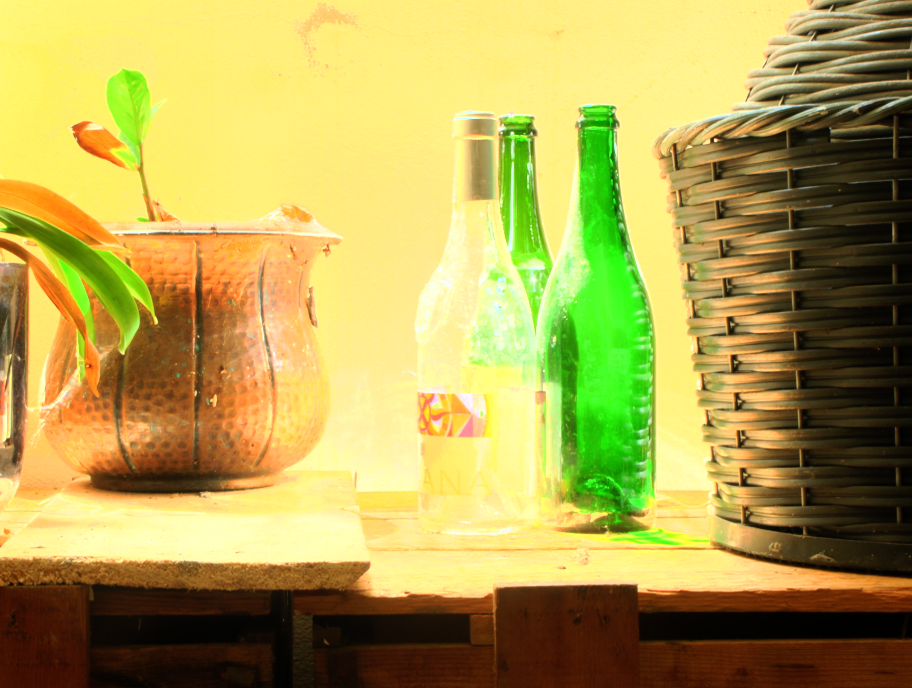
\includegraphics[height=1.5cm]{Imagens/Bottles_Small-ETM.png}}
%    \hspace{0.3cm}
%  \subfloat[METM]{\label{fig:METM} 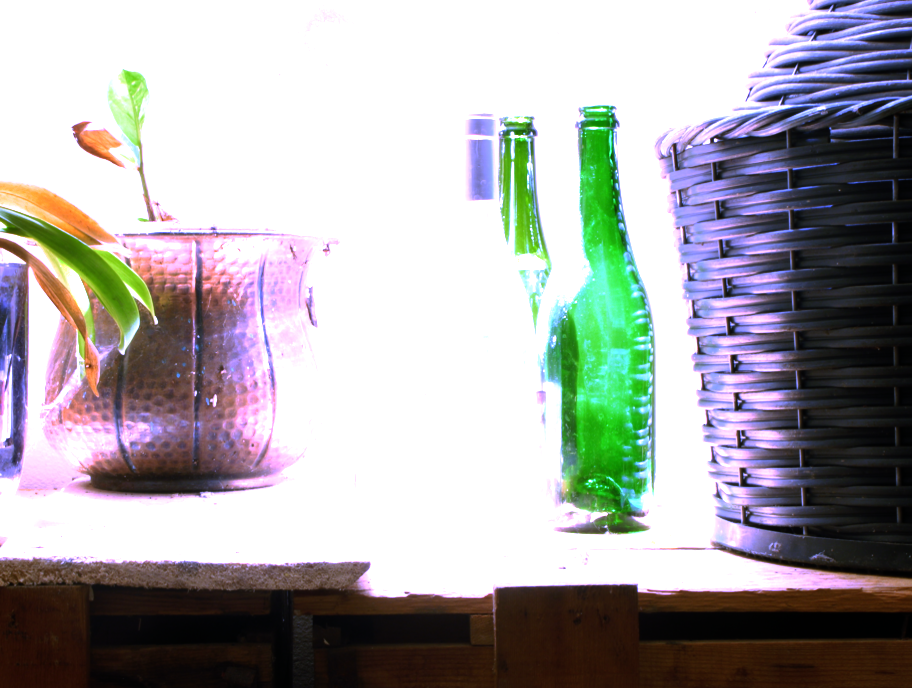
\includegraphics[height=1.5cm]{Imagens/Bottles_Small-METM.png}}
%  \hspace{0.3cm}
%   \subfloat[LTM]{\label{fig:LTM}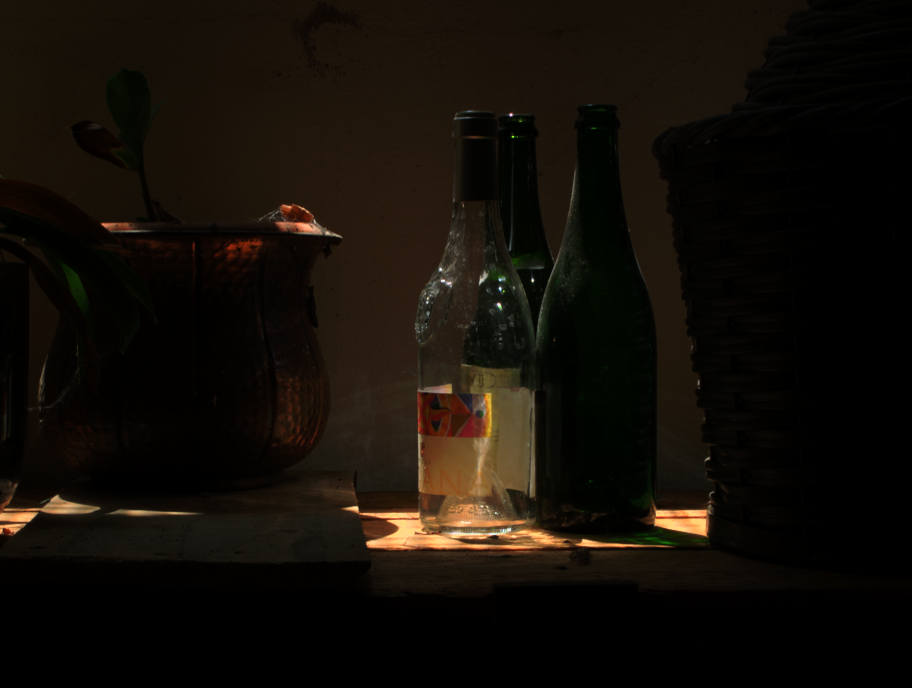
\includegraphics[height=1.5cm]{Imagens/Bottles_Small-LTM.png}}
%    \hspace{0.3cm}
%   \subfloat[MLTM]{\label{fig:MLTM}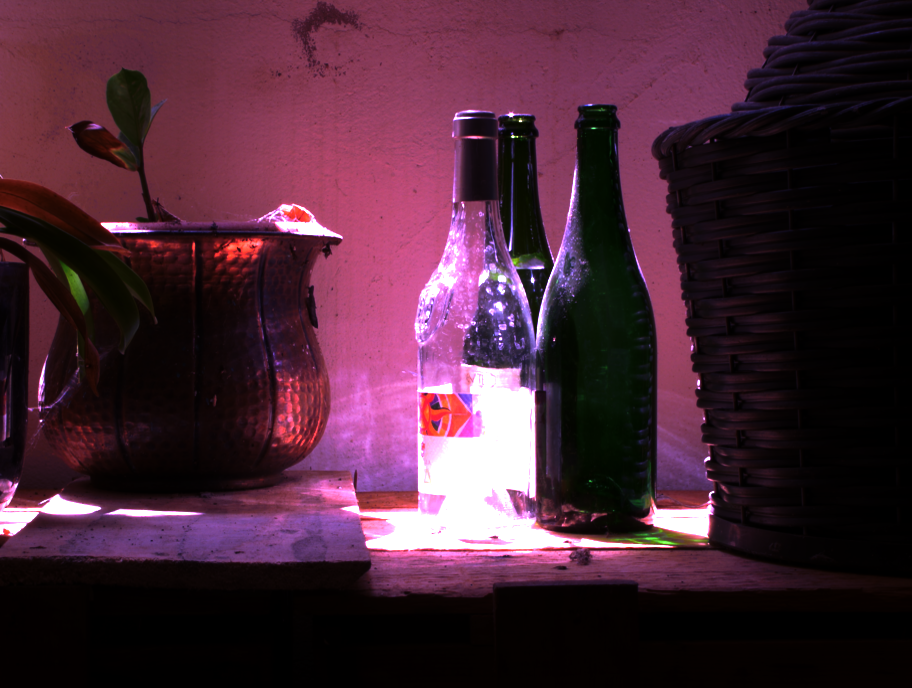
\includegraphics[height=1.5cm]{Imagens/Bottles_Small-MLTM.png}}
%    \caption{Bottles Small}
%    \label{fig:bS}
%\end{figure}

%\begin{figure}[!htp]
%   \centering
%  \subfloat[ETM]{\label{fig:ETM}\includegraphics[height=1.5cm]{Imagens/Iwate-ETM.png}}
%    \hspace{0.3cm}
%  \subfloat[METM]{\label{fig:METM} \includegraphics[height=1.5cm]{Imagens/Iwate-METM.png}}
%  \hspace{0.3cm}
%   \subfloat[LTM]{\label{fig:LTM}\includegraphics[height=1.5cm]{Imagens/Iwate-LTM.png}}
%    \hspace{0.3cm}
%   \subfloat[MLTM]{\label{fig:MLTM}
\includegraphics[height=1.5cm]{Imagens/Iwate-MLTM.png}}
%    \caption{Iwate}
%    \label{fig:iT}
%\end{figure}

%\begin{figure}[!htp]
%   \centering
%  \subfloat[ETM]{\label{fig:ETM}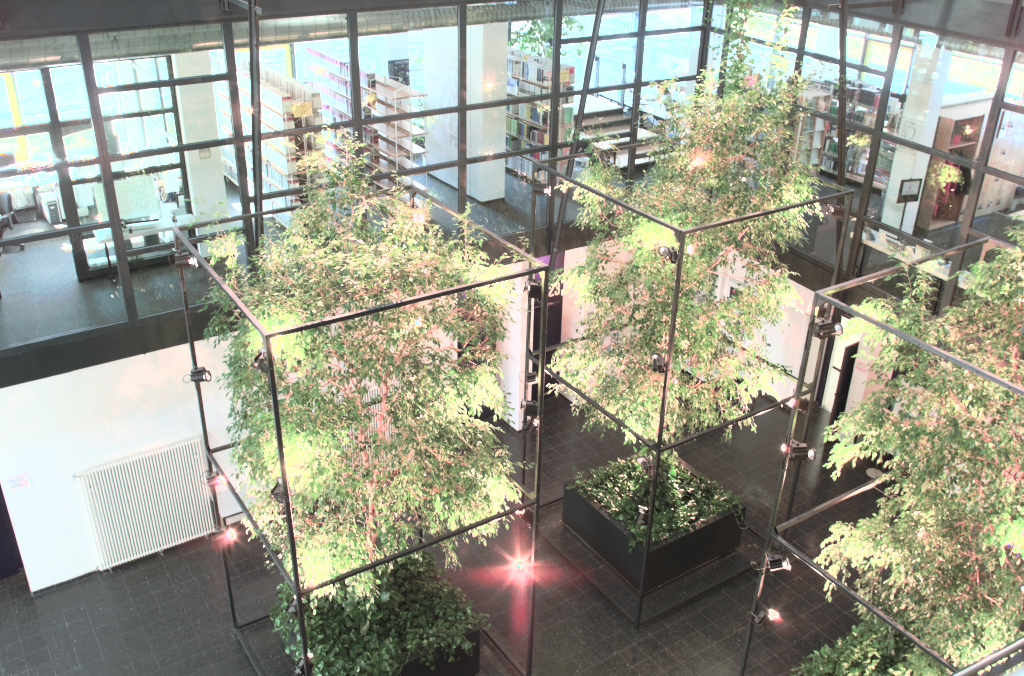
\includegraphics[height=1.5cm]{Imagens/mpi_atrium_1-ETM.png}}
%    \hspace{0.3cm}
%  \subfloat[METM]{\label{fig:METM} 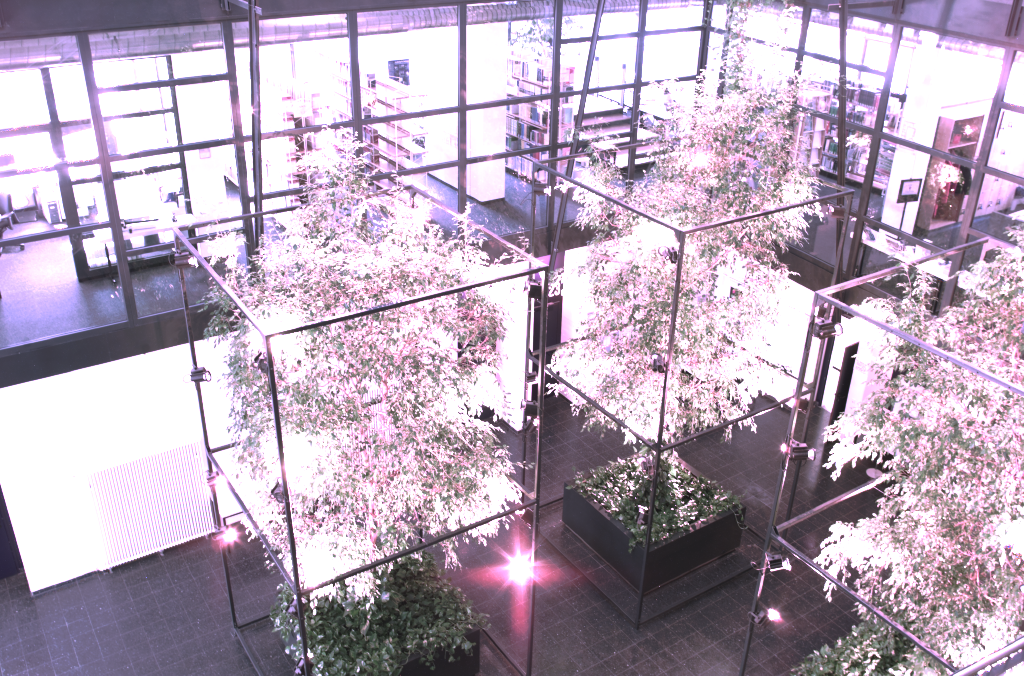
\includegraphics[height=1.5cm]{Imagens/mpi_atrium_1-METM.png}}
%  \hspace{0.3cm}
%   \subfloat[LTM]{\label{fig:LTM}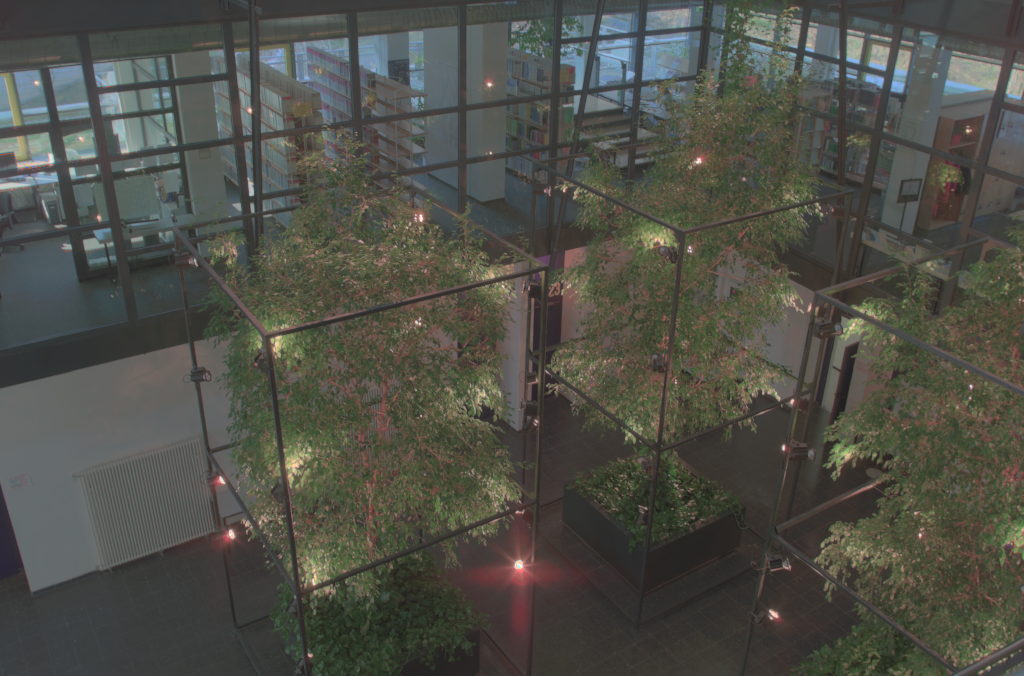
\includegraphics[height=1.5cm]{Imagens/mpi_atrium_1-LTM.png}}
%    \hspace{0.3cm}
%   \subfloat[MLTM]{\label{fig:MLTM}
\includegraphics[height=1.5cm]{Imagens/mpi_atrium_1-MLTM.png}}
%    \caption{MPI Atrium}
%    \label{fig:mA}
%\end{figure}

%\begin{figure}[!htp]
%   \centering
%  \subfloat[ETM]{\label{fig:ETM}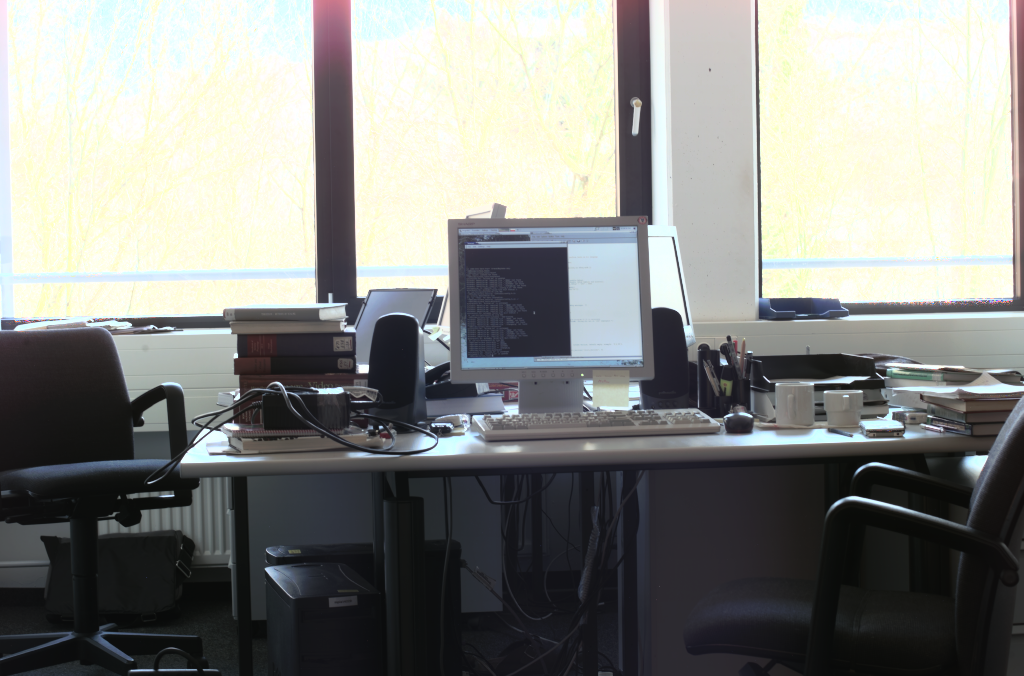
\includegraphics[height=1.5cm]{Imagens/mpi_office-ETM.png}}
%    \hspace{0.3cm}
%  \subfloat[METM]{\label{fig:METM} 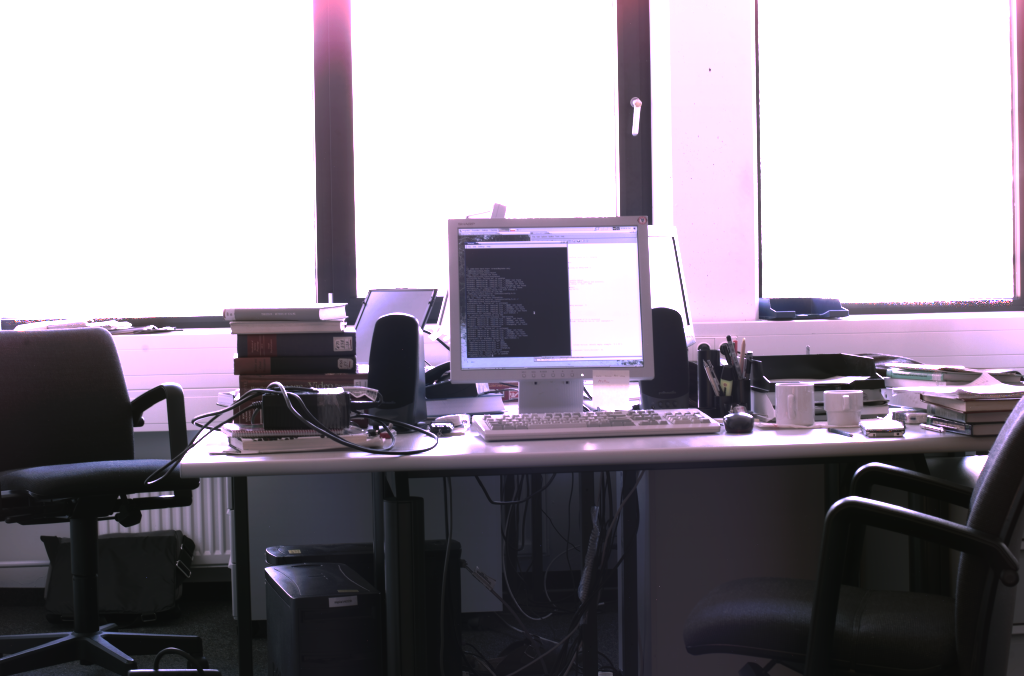
\includegraphics[height=1.5cm]{Imagens/mpi_office-METM.png}}
%  \hspace{0.3cm}
%   \subfloat[LTM]{\label{fig:LTM}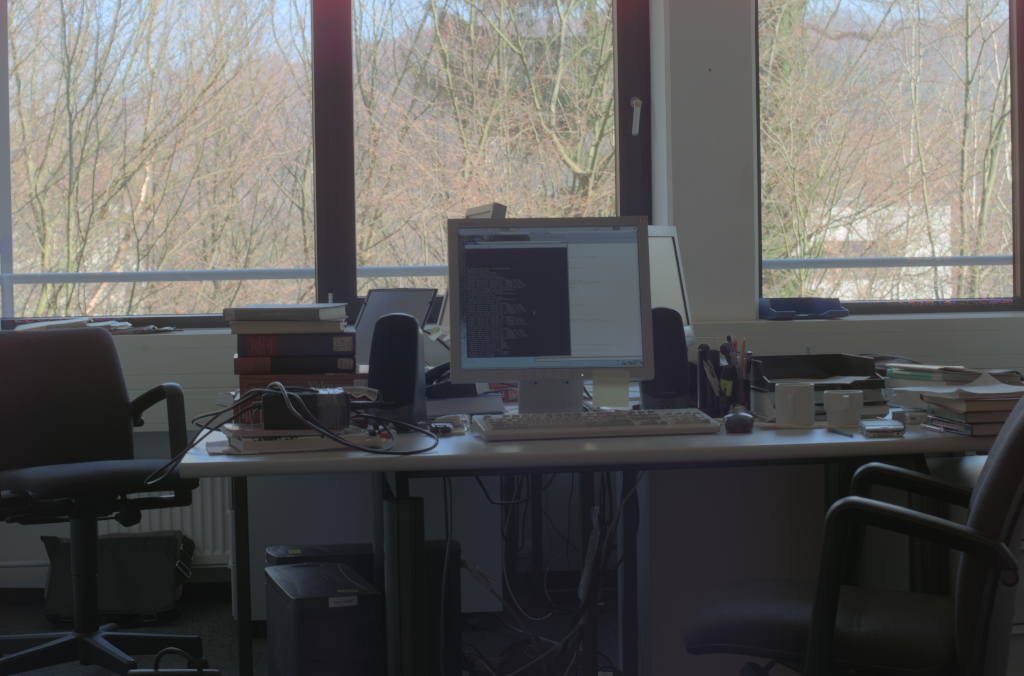
\includegraphics[height=1.5cm]{Imagens/mpi_office-LTM.png}}
%    \hspace{0.3cm}
%   \subfloat[MLTM]{\label{fig:MLTM}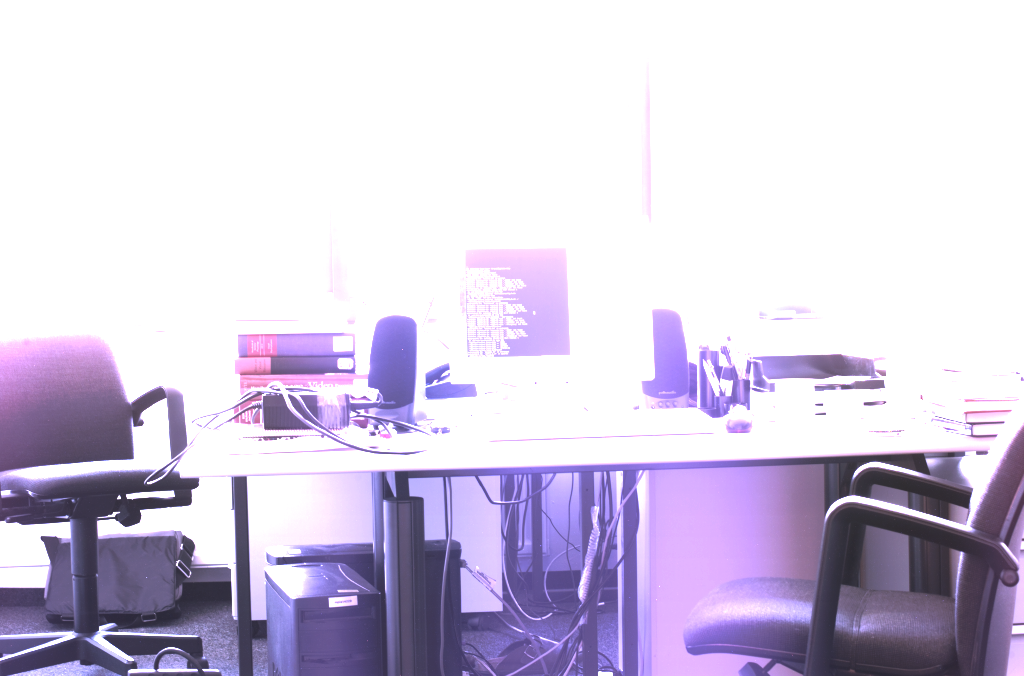
\includegraphics[height=1.5cm]{Imagens/mpi_office-MLTM.png}}
%    \caption{MPI Office}
%    \label{fig:mO}
%\end{figure}

%\begin{figure}[!htp]
%  \centering
%  \subfloat[ETM]{\label{fig:ETM}\includegraphics[height=1.5cm]{Imagens/nancy_cathedral_1-ETM.png}}
%    \hspace{0.3cm}
%  \subfloat[METM]{\label{fig:METM} \includegraphics[height=1.5cm]{Imagens/nancy_cathedral_1-METM.png}}
%  \hspace{0.3cm}
%   \subfloat[LTM]{\label{fig:LTM}\includegraphics[height=1.5cm]{Imagens/nancy_cathedral_1-LTM.png}}
%    \hspace{0.3cm}
%   \subfloat[MLTM]{\label{fig:MLTM}
\includegraphics[height=1.5cm]{Imagens/nancy_cathedral_1-MLTM.png}}
 %   \caption{Nancy Cathedral 1}
  %  \label{fig:nc1}
%\end{figure}

%\begin{figure}[!htp]
 %  \centering
 % \subfloat[ETM]{\label{fig:ETM}\includegraphics[height=1.5cm]{Imagens/nancy_cathedral_2-ETM.png}}
 %   \hspace{0.3cm}
 % \subfloat[METM]{\label{fig:METM} \includegraphics[height=1.5cm]{Imagens/nancy_cathedral_2-METM.png}}
 % \hspace{0.3cm}
 %  \subfloat[LTM]{\label{fig:LTM}\includegraphics[height=1.5cm]{Imagens/nancy_cathedral_2-LTM.png}}
 %   \hspace{0.3cm}
 %  \subfloat[MLTM]{\label{fig:MLTM}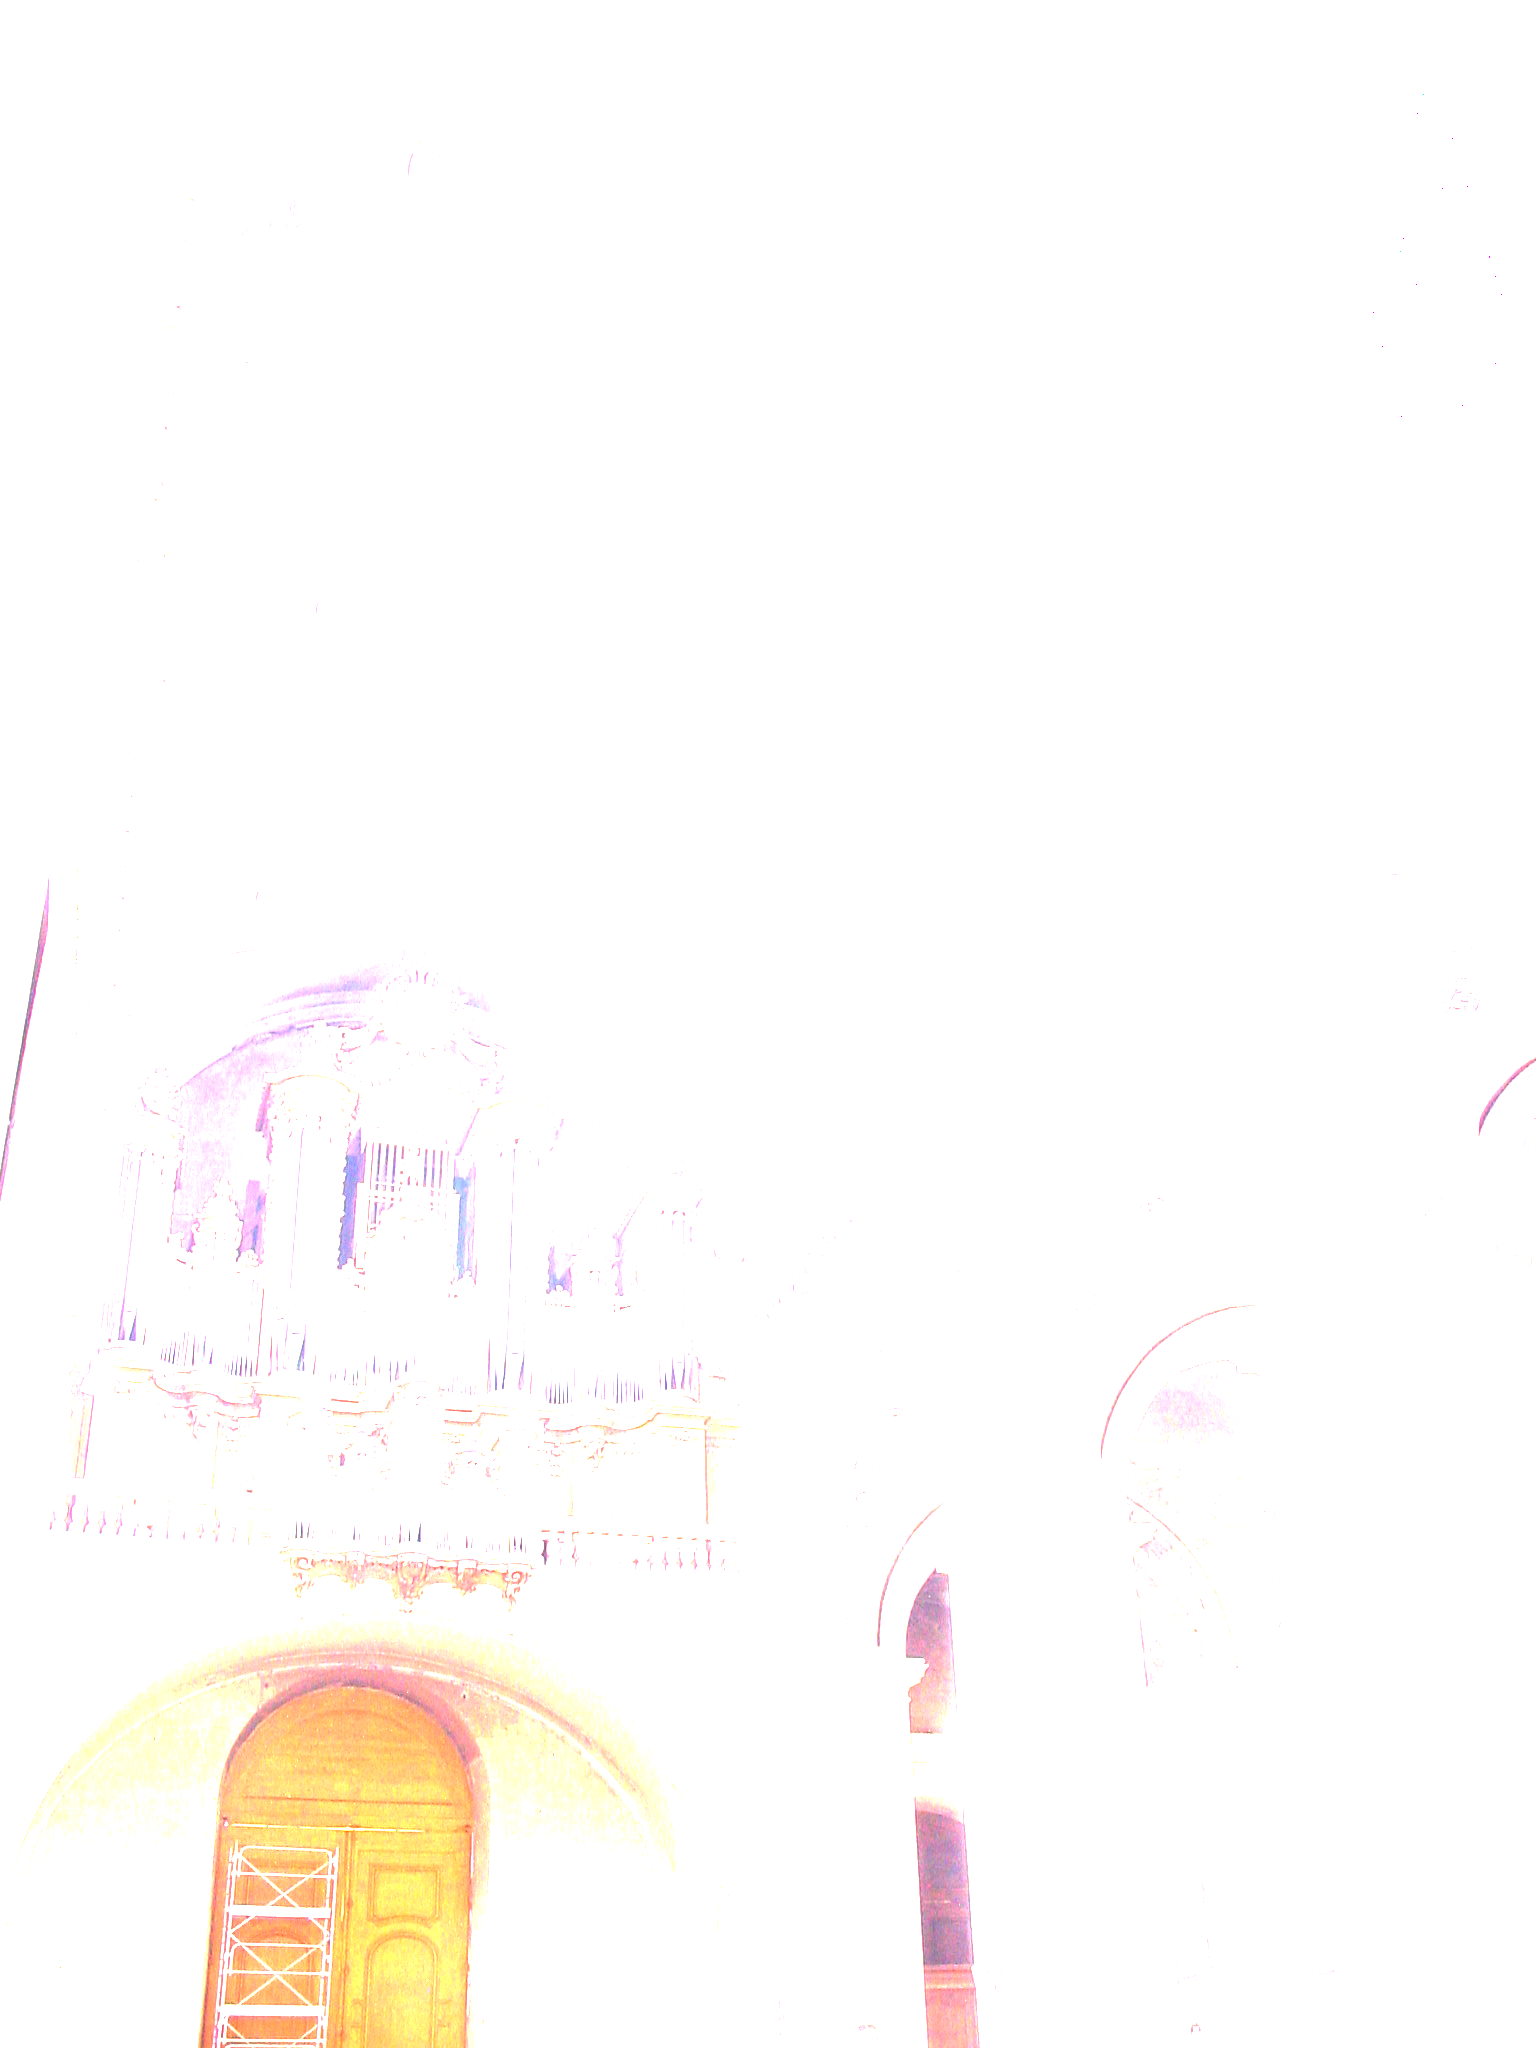
\includegraphics[height=1.5cm]{Imagens/nancy_cathedral_2-MLTM.png}}
 %   \caption{Nancy Cathedral 2}
 %   \label{fig:nc2}
%\end{figure}

%\begin{figure}[!htp]
%   \centering
%  \subfloat[ETM]{\label{fig:ETM}\includegraphics[height=1.5cm]{Imagens/nancy_church_1-ETM.png}}
 %   \hspace{0.3cm}
%  \subfloat[METM]{\label{fig:METM} \includegraphics[height=1.5cm]{Imagens/nancy_church_1-METM.png}}
%  \hspace{0.3cm}
%   \subfloat[LTM]{\label{fig:LTM}\includegraphics[height=1.5cm]{Imagens/nancy_church_1-LTM.png}}
%    \hspace{0.3cm}
%   \subfloat[MLTM]{\label{fig:MLTM}\includegraphics[height=1.5cm]{Imagens/nancy_church_1-MLTM.png}}
%    \caption{Nancy Church}
%    \label{fig:ncc}
%\end{figure}

%\begin{figure}[!htp]
%   \centering
%  \subfloat[ETM]{\label{fig:ETM}\includegraphics[height=1.5cm]{Imagens/seymour_park-ETM.png}}
%    \hspace{0.3cm}
%  \subfloat[METM]{\label{fig:METM} \includegraphics[height=1.5cm]{Imagens/seymour_park-METM.png}}
%  \hspace{0.3cm}
%  \subfloat[LTM]{\label{fig:LTM}\includegraphics[height=1.5cm]{Imagens/seymour_park-LTM.png}}
%    \hspace{0.3cm}
%   \subfloat[MLTM]{\label{fig:MLTM}
\includegraphics[height=1.5cm]{Imagens/seymour_park-MLTM.png}}
%    \caption{Seymour Park}
%    \label{fig:sP}
%\end{figure}

%\begin{figure}[!htp]
%   \centering
%  \subfloat[ETM]{\label{fig:ETM}\includegraphics[height=1.5cm]{Imagens/snow-ETM.png}}
%    \hspace{0.3cm}
%  \subfloat[METM]{\label{fig:METM} \includegraphics[height=1.5cm]{Imagens/snow-METM.png}}
%  \hspace{0.3cm}
%   \subfloat[LTM]{\label{fig:LTM}\includegraphics[height=1.5cm]{Imagens/snow-LTM.png}}
%    \hspace{0.3cm}
%   \subfloat[MLTM]{\label{fig:MLTM}\includegraphics[height=1.5cm]{Imagens/snow-MLTM.png}}
%    \caption{Snow}
%    \label{fig:sW}
%\end{figure}
%---------------------------------------------------------

\begin{figure}[!htpb]
    \centering
    \includegraphics[scale=.20]{Imagens/comp.jpg}
    \caption{Comparação dos Quality Score entre Antrium Night e Antrium Morning}
    \label{comp}
\end{figure}
No gráfico da Figura \ref{comp}, é possível visualizar que o \textit{Quality Score} é superior nos algoritmos de LTM. Porém a diferença dele para ETM e METM são dadas como inferiores a 10\%, indo de encontro com os resultados obtidos na análise subjetiva, aonde a diferença da qualidade não aparenta ser tão pequena.

O que pode ser observado ao comparar as imagens, é que as resultantes do operador LTM foram as que melhor representaram a granularidade dos detalhes da imagem, sem muito estouro de branco, fazendo com que os pontos não se sobressaíssem, e causando um efeito de flare na imagem. Ao contrário dos resultados dos outros operadores, em que essas aberrações cromáticas acontecem com maior frequências, causando um impacto nas cores, que ficam muito mais próximos de uma escala de branco, com alguns pontos se realçando por não receberem essa claridade excessiva, mas acabando ficando com pouco realce e perdendo detalhes.

Esse efeito pode ser visto na Figura \ref{esc}, aonde na área circulada é possível perceber existência da uma porta na primeira imagem (LTM), enquanto a mesma área na segunda imagem (ETM) é muito escura, não permitindo visualizar a porta.

\begin{figure}[!htpb]
    \centering
    \includegraphics[scale=.20]{Imagens/ima.jpg}
    \caption{Pontos mais escuros em comparação LTM e ETM}
    \label{esc}
\end{figure}

O código fonte implementado para o trabalho, todas as figuras resultantes da execução e todos os valores da avaliação TMQI podem ser encontrados no Github\footnote{https://github.com/hpfred/Octave-Tone-Mapping-and-Quality-Index-Implementations}, ou alternativamente acessando o Drive\footnote{https://drive.google.com/drive/u/2/folders/1hWx2gS6fRS6cTUzci5F8UfjizimUEdi7} (para acesso ao Drive é necessário o uso do e-mail institucional).

\section{Conclusão}

A popularização do uso do \textit{High Dynamic Range} (HDR), incluindo sua presença ubíqua nas câmeras de aparelhos celulares modernos vem fomentando o interesse e investimento em pesquisas na área, muito disso sendo o estudo dos algoritmos de Tone Mapping que melhor traduzem a imagem original em LDR.

Com o objetivo de implementar algoritmos capazes de nos auxiliar a visualizar essas imagem HDR, utilizamos das diferentes técnicas de \textit{Tone Mapping}, com os métodos globais Logarítmico (LTM), Logarítmico Modificado (MLTM), Exponencial (ETM) e Exponencial Modificado (METM). Essa implementação foi realizada seguindo os exemplos do trabalho de ~\cite{ICIAS}, no qual nos apresenta alguns operadores de \textit{Tone Mapping}, juntamente com fórmulas da implementação dos mesmos. Porém durante as implementações, foram identificados problemas na representação de algumas dessas fórmulas, sendo assim necessário recorrer a outras implementações como \cite{TMLib} e \cite{Duarte:2016}, para então compreender aonde cada uma carecia na sua implementação e documentação, e então juntar o conhecimento de todas para obter uma implementação simples e funcional.

Ao realizar a execução dos algoritmos desenvolvidos, foi possível visualizar que alguns dos operadores resultava em imagens um pouco diferentes do esperado, mas não chegamos a ter tempo suficiente para testar modificar valores de parâmetros para ver como isso modificaria as imagens resultantes. Porém ainda tivemos problemas com o operador METM, no qual não só destoou do esperado, como também todos resultados apresentaram um tom de cor mais roxo, e com o operador MLTM, que apresentou um estouro de branco nos seus resultados, sendo impossível de visualizar qualquer detalhe na maioria das imagens resultantes, com apenas algumas delas apresentando os pontos mais escuros visíveis.

Para auxiliar na análise dessas imagens foi utilizada uma implementação da função TMQI, onde foi possível realizar uma comparação entre a imagem original em HDR e a gerada pelos métodos. Ao término dessa comparação foram gerados arquivos .txt, para assim apresentar todos os resultados gerados. A análise desses arquivos de texto permitiram perceber que os resultados do \textit{Quality Score} apresentam um valor objetivamente melhor para o operador Logarítmico, algo também comprovado pelo teste de análise visual, realizado pelos integrantes deste trabalho.

Dessa forma, após todos os desafios encontrados pelo uso do Octave no lugar do Matlab, além dos desafios comumente encontrados em qualquer implementação de trabalho, foi possível obter um melhor entendimento do conteúdo da cadeira de Processamento Digital de Imagens (PDI) e principalmente da sub-área de tratamento de imagens HDR, e compilar esse conhecimento da melhor forma possível neste artigo para talvez auxiliar pessoas pesquisando o mesmo assunto no futuro.

\bibliographystyle{IEEEtran}
\bibliography{referencias.bib}

%\begin{thebibliography}{00}
%\bibitem{b1} G. Eason, B. Noble, and I. N. Sneddon, ``On %certain integrals of Lipschitz-Hankel type involving products %f Bessel functions,'' Phil. Trans. Roy. Soc. London, vol. %A247, pp. 529--551, April 1955.
%bibitem{b2} J. Clerk Maxwell, A Treatise on Electricity and %agnetism, 3rd ed., vol. 2. Oxford: Clarendon, 1892, %p.68--73.
%\bibitem{b3} I. S. Jacobs and C. P. Bean, ``Fine particles, %thin films and exchange anisotropy,'' in Magnetism, vol. III, %. T. Rado and H. Suhl, Eds. New York: Academic, 1963, pp. %271--350.
%\bibitem{b4} K. Elissa, ``Title of paper if known,'' %unpublished.
%\bibitem{b5} R. Nicole, ``Title of paper with only first word %capitalized,'' J. Name Stand. Abbrev., in press.
%\bibitem{b6} Y. Yorozu, M. Hirano, K. Oka, and Y. Tagawa, %``Electron spectroscopy studies on magneto-optical media and %plastic substrate interface,'' IEEE Transl. J. Magn. Japan, %vol. 2, pp. 740--741, August 1987 [Digests 9th Annual Conf. %Magnetics Japan, p. 301, 1982].
%\bibitem{b7} M. Young, The Technical Writer's Handbook. Mill %Valley, CA: University Science, 1989.
%\bibitem{}
%\end{thebibliography}
\vspace{12pt}

\end{document}
